\chapter{Dynamic Systems and Control}

\section{Introduction}

(from introduction)

"Considering that any currency mechanism is absent from this model of sup-
ply and demand is seems reasonable to find a way to include currency in our
model. This leads to the question of what methods should be used to analyze
the properties of currency."

"The fundamental insight that we present is that because currency is a digital
system, the way to approach its analysis is roughly analogous to the way we
approach the analysis and design of other digital systems (the internet being an
interesting case in point), i.e. that we should approach the analysis of currency
as an engineering problem, and in particular the engineering and control of
dynamic systems."

In this chapter we introduce foundations for an engineering analysis of currency. Dynamic systems
and control system engineering are a broad, over-arching engineering disciples relevant across
virtually all more specialized disciplines. We require a good understanding of negative feedback,
positive feedback, PID controllers, the effects of noise and errors on systems and design responses
to handle noise and errors.

We do not use an engineering approach for the analysis of the equilibriation process observed in
markets. The only rule the we accept governs market behaviour is the lawx of supply and demand only
at an aggregate level, as was so nicely described by David Hume. The only assumption we make about
the law of supply and demand at an aggregate level is that the price level and quantities and goods
and services adjust to the point where aggregate excess supply or aggregate excess demand tend to
zero. We only accept this assumption to the extent that it can be empirically justified.

% Chapter:          Dynamic Systems and Control
% Secion:           Negative Feedback
\section{Negative Feedback}

Negative feedback is a process of repetitively measuring by how much a system deviates from a
desired value, and feeding that error back into the system in proportion to the degree of the error. 





We are looking for a way that we can keep the conditions of the system in some desirable state.
Examples are ... If the system is predictable can use an open system. Many systems, however are not
completely predictable. In many case, despite the unpredictability we can still control the system
to a certain degree. One method is to use a closed system. Another method is to introduce a
sophisticated controller into the loop, such as a human, in combination with the mechanism. Examples
are ...

A heater with a fixed output.

A heater with a thermostat.

Using a schema similar to \ref{fig:feedback_schema} we can represent the cyclist as,

\begin{figure}
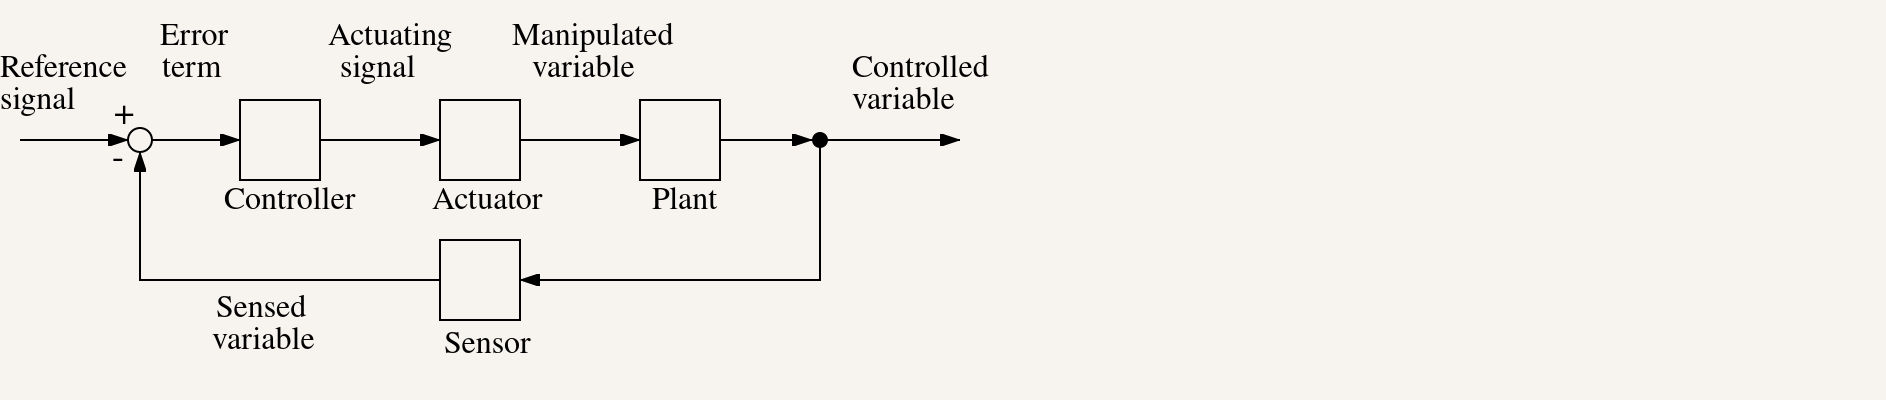
\includegraphics[scale=0.48]{/02/bicycle_feedback_schema}
\caption{Bicycle Feedback Schema}
\label{fig:bicycle_feedback_schema}
\end{figure}

The 'reference signal' or 'set point' is the goal of the system, in this case most likely a
desination and when they want to arrive. The controller takes the set point and the present
conditions, i.e. where the cyclist is currently, the location of obstacles, if the road is heading
uphill or downhill etc.  weather conditions are, how much time they have remaining and convert this
into a control signal. Part of the control signal in this case is observable - the person's
adjustments to the handle-bars, other signals are not observable such as decisions on how hard to
pedal. The actuator in this case is the cyclists leg muscles, which convert those desicions, and use
energy to convert them into pedal pressure. The cyclist then observes the situation again and reacts
to the situation by feeding their sensory data back into the 'controller' and so on in a closed
loop. In the case of the cyclist we depend on continuous inputs in a changing, often unpredictable
environment to adjust behaviour - we require a closed loop system.

\subsubsection{Huygens}

\subsubsection{Watt}

\subsection{PID controller}

\subsubsection{James Clerk Maxwell}

\subsubsection{The Wright Brothers}

Prior to the Wright brother's first flight in December 1903, Orville and Wilbur Wright believed that
the most fundamental problems they needed to solve were control problems. In September 1901 Wilbur
Wright's first public presentation on the feasibility of heavier-than-air flight stated that ``When
this one feature [control] has been worked out the age of flying machines will have arrived, for all
other difficulties are of minor importance."\cite{wright1908}

% TODO - this paragraph requires work.

The general view prior to the Wright brothers was that aircraft required the mechanism to
self-stabilize. [this was a problem because incorporating stability into the air-craft was at the
cost of agility. Possibly because the Wright brothers were bicycle-shop owners, and were aware that
bicycles are fundamentally unstable and require human intervention to stay upright, they understood
that this control could be done by the pilot rather than the plane.

\subsubsection{Elmer Sperry}

Elmer Sperry was the first to construct a PID controller. One notable characteristic of PID
controllers is that despite much work in the design of more sophisticated controllers, PID
controllers are by far the most widely used, demonstrating robustness to solve a broad range of
control problems.

Elmer Sperry is best known for his construction and application of gyroscopes following the
invention of the first practical gyroscope by Hermann Anschütz-Kaempfe in 1904. One of Sperry's
applications was the use of a gyroscope as a component in a control system to self-stabilize
airplanes.

[longer flights]
 
Following on from these experiences, he worked with the U.S. Navy to use gyroscopes for stabilizing
ships, and then also to build control systems as auto-pilots of ships. Because the control process
involved in steering large ships with significant lags and so was relative slow and visible, he was
able to observe that skilled helmsmen used a more nuanced 'algorithm' than just a proportional
response, and that the helmsman with put the helm over in the opposite to the directions in which
the ship was yawing a significantly in advance (a D response), and that helmsman worked the ship
upwards in response to currents and prevailing wind (an I response). Sperry then incorporated these
three responses (P, I and D) into his mechanical control mechanism which connected the gyroscope to
the ships steering.

In 1922 Nicolas Minorsky published a paper which encapsulated the P, I and D into an
equation.\cite{minorsky1922}

% chapter:          Dynamic Systems
% section:          Positive Feedback
\section{Positive Feedback}

% chapter:          Dynamic Systems
% section:          Error Correction
\section{Error Correction}

% chapter:          Dynamic Systems
% section:          Isolation 
\section{Isolation}

% chapter:          Dynamic Systems
% section:          Stability
\section{Stability}

% chapter:          Dynamic Systems
% section:          Internet
\section{Internet}

% chapter:          Dynamic Systems
% section:          Internet
% subsection:       Introduction
\subsection{Internet::Introduction}

% chapter:          Dynamic Systems
% section:          Internet
% subsection:       Introduction
% subsubsection:    Some Abstractions - Multiplexing
\subsubsection{Some Abstractions - Multiplexing}

% chapter:          Dynamic Systems
% section:          Internet
% subsection:       Introduction
% subsubsection:    Packet Switching 
\subsubsection{Packet Switching}

The most notable difference between digital networks and the precursor to digital networks - the
telephone network - was the notion of packet switching.

% Baran

In the mid 1960s Paul Baran was working on the problem of fault-tolerant networks\cite{baran1964intro}.

\begin{quote}
Packet switching technology was not really an invention, but a reapplication of the basic
    dynamic-allocation techniques used for over a century by the mail, telegraph, and torn paper
    tape switching systems. \cite{roberts1978}
\end{quote}

% Pre-allocation

radio, telephony

Analog telephone systems work by setting up a connection between two telephones. This connection
takes complete ownership of the physical connection, the wire. Baran proposed to share the physical
wire between many connections. Time division multiplexing had been used since the late 19th century
to share a single wire to send multiple telegraph messages synchronously. This was called time
division multiplexing. The idea was to share the wire by allocating divisions of time for each
message. Baran's idea was rather than to multiplex by time, to multiplex by a standardized message
block, later termed a 'packet'.

% Dynamic allocation

telegraph and mail systems

\begin{quote}
Time division multiplexing appears so natural to data transmission that we might wish to consider an
alternative approach -- a standardized message block as a network interface standard.\cite{baran1964intro}
\end{quote}

The reasons were

% Efficiency

telephone systems multiplex, i.e. chop up and share out communication by pre-allocating transmission
bandwidth a connect (or telephone call). Data transmission comes in short bursts, so the complete
physical connection is 'blocked' by the empty parts in a transmission, and so roughly 90 percent of
capacity was wasted. We can see why telegraphy was so much cheaper than voice communication. By
reducing the granularity of the chopping-up into small packets, one could more efficiently share out
the resource, by filling up the blank spaces by some other communication.

% Reliability

% Dynamics

A telephone call fixes the relationship between transmitted information and the network. By
packaging up information and assigning each package a destination address, a degree of freedom is
introduced between the transmitted information and the network. This means that information can be
rerouted, i.e. respond to network conditions, directly attacking the problem of network fault
tolerance. We have introduced a negative feedback here, i.e. a response to failure in the network,
so as to maintain a stable condition i.e. the success rate of transmissions. We'll look at how this
is implemented in section A.

Such dynamic systems require feedback for regulation.

% chapter:          Dynamic Systems
% section:          Internet
% subsection:       Introduction
% subsubsection:    Some Abstractions - Hiding 
\subsubsection{Some Abstractions - Hiding}

% TODO: Need a 'hindsight' qualification.

% chapter:          Dynamic Systems
% section:          Internet
% subsection:       Introduction
% subsubsection:    Some Constraints - Distributed Systems 
\subsubsection{Some Constraints - Distributed Systems}

\subsubsection{Some Constraints - Burstiness}

\subsubsection{Some Constraints - Heterogenous Networks and Hardware}

In the early 1970s a protocol for joining together many networks. The question is why would you
join together networks, each with their own hardware and protocols? Why not select a uniform
protocol that is universal across all networks?

\begin{quote}
    Even though many different and complex problems must be solved in the design of an individual
    packet switching network, these problems are manifestly compounded when dissimilar networks are
    interconnected. Issues arise which may have no direct counterpart in an individual network and
    which strongly influence the way in which internetwork communication can take place.
    \cite{cerf1974}
\end{quote}

% TODO: Answer this question

% This section should probably be shifted to a later section.

The main problem of building a network of networks, i.e. the internet was to figure out a way for
many different kinds of networks to interoperate. In the foundational paper outlining how to
approach this problem\cite{cerf1974}, Cerf and Kahn utilize the hiding abstraction as much as
possible, to reduce the complexity of interactions between the different networks. In the abstract
they enumerate the functionality to be passed off to individual networks, 

\begin{quote}
The protocol provides for variation in individual network packet sizes, transmission failures,
sequencing, flow control, end-to-end error checking, and the creation and destruction of logical
process-to-process connections.
\end{quote}

This could be summarized as passing off dynamic feedback to the individual networks, and specifying
the minimum static properties that all networks must share. 


% Re-check this quote - it might be out of context.
\begin{quote}
    [Systems] such as real-time traffic that can adapt its sending rate to reduce loss and/or delay
    [are] most effective when the adaption occurs on timescales of a single Round-Trip Time (RTT) or
    a small number of RTTs, for elastic traffic.\cite{rfc7567}, page 6.
\end{quote}

% chapter:          Dynamics Systems
% section:          Internet
% subsection:       TCP/IP
\subsection{TCP/IP}

% TODO: Description of IP

% TODO: Description of TCP

% TODO: Historical process of separating out TCP and IP. (see Roberts)

% TODO: We want to show that IP is the plant and that TCP is feedback.
% 

% chapter:          Dynamic Systems
% section:          Internet
% subsection:       TCP/IP
% subsubsection:    Control System Components
\subsubsection{Control System Components}

\begin{figure}
\includegraphics[scale=0.28]{/01/feedback_schema}
\caption{Control System Schema}
\label{fig:feedback_schema}
\end{figure}

% chapter:          Dynamic Systems
% section:          Internet
% subsection:       Congestion
\subsection{Congestion}

% chapter:          Dynamic Systems
% section:          Internet
% subsection:       Congestion
% subsubsection:    TCP Feedback schema 
\subsubsection{TCP Feedback Schema} 

What should the set-point be?

\begin{quote}
The naive assumption might be that there is a simple trade-off between delay and throughput, and
that the recommendation that queues be maintained in a "non-full" state essentially translates
to a recommendation that low end-to-end delay is more important than high throughput. However,
this does not take into account the critical role that packet bursts play in Internet
performance. For example, even though TCP constrains the congenstion window of a flow, packets
often arrive at network devices in bursts [Leland94]. If the queue is full or almost full, an
arriving burst will cause multiple packets to be dropped from the same flow. Bursts of loss can
result in a gloabl synchronization of flows throttling back, followed by a sustained period of
lowered link utilixzation, reducing overall throughput. \cite{rfc7567} page 8.
\end{quote}

What information should be transmitted?

\begin{quote}
By means of simulating TCP/IP network operations we are able to examine in detail the causes of
traffic oscillation in a simple network setting. Our analysis shows that users' control actions
are highly synchronized by the network congestion signaling and that providing users only a
    binary network state can lead to repeated oscillations\cite{zhang1990}.
\end{quote}


% TODO: Check references [Leland94], [Flo94], [Zha90].

% chapter:          Dynamic Systems
% section:          Internet
% subsection:       Congestion
% subsubsection:    The Actual Design
\subsection{The Actual Design}

% TODO: Place this image in the correct place

\begin{figure}
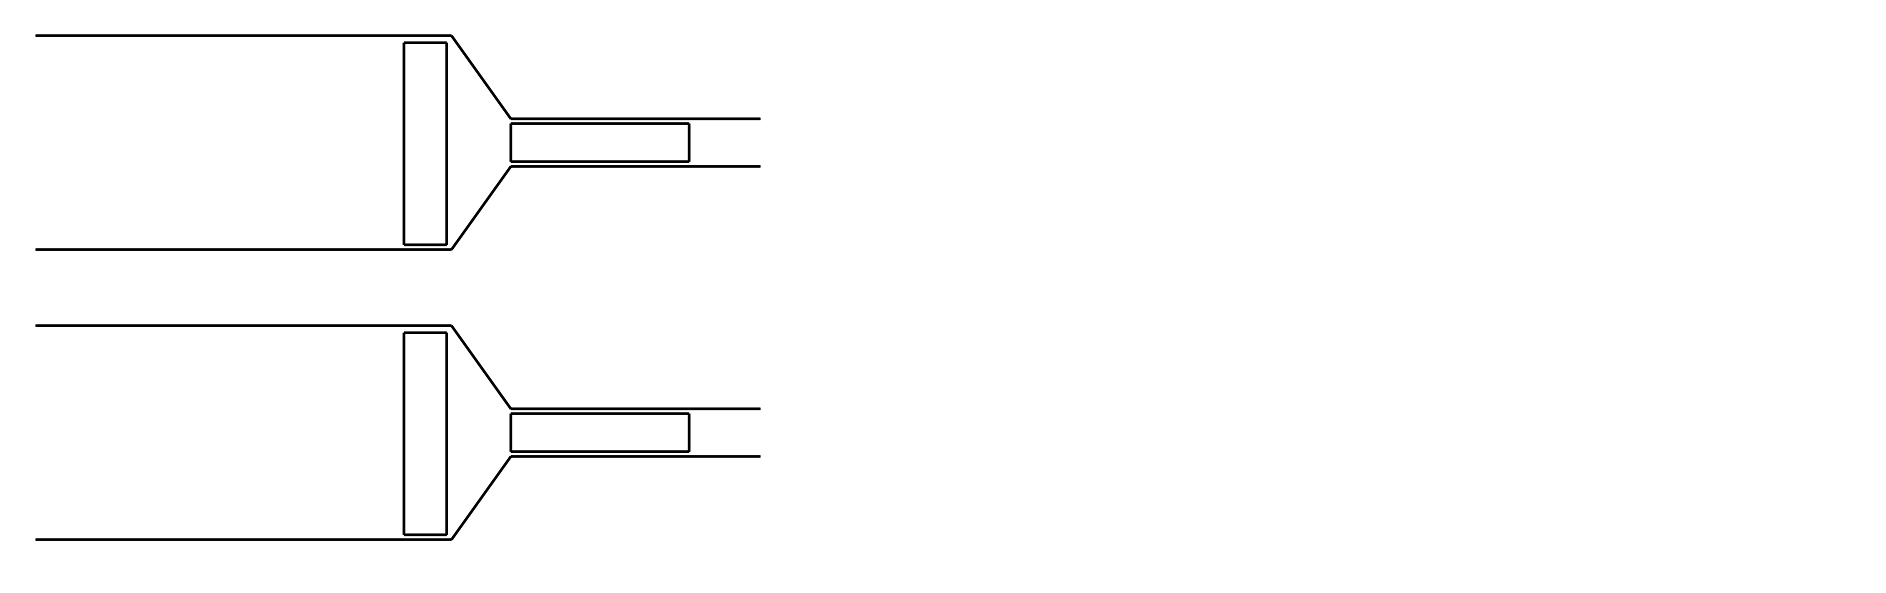
\includegraphics[scale=0.48]{/02/bandwidth_transition}
\caption{Packets reaching bandwith transition}
\label{fig:bandwidth_transition}
\end{figure}


% ACK clocking is pseudo-mechanical. When this system was designed the cost (monetary and in time)
% of computer processing was large. The IMP (the interface 'card') had 12K of memory and a cost of
% hundreds of thousands of dollars. The ingenuity of mechanical feedback stabilization mechanism is
% remarkable, and given the costs at the time, made sense. In general though, mechanical feedback
% processes are highly inflexible (hence the ingenuity required) compared to a simple PID
% controller.   

\subsubsection{History of "Tail-Drop" Queueing}

\begin{quote}
The traditional technique for managing the queue length in a network device is to set a maximum
    length (in terms of packets) for each queue, accept packets for the queue until the maximum
    length is reached, then reject (drop) subsequent income packets until the queue decreases
    because a packet from the queu has been transmitted. This technique is known as "tail drop",
    since the packet that arrived most recently (i.e. the one on the tail of the queue) is dropped
    when the queue is full. This method has served the Internet well for years, but it has four
    imporant drawbacks. \cite{rfc7567} p. 8.
\end{quote}

The first being,

\begin{quote}
The "tail drop" discipline allows queues to maintain a full (or almost full) status for long periods
of time, since tail drop signals congestion (via a packet drop) only when the queue has become
full. It is important to reduce the steady-state queue size, and this is perhaps the most
important goal for queue management. \cite{rfc7567} p. 8.
\end{quote}

% TODO: This is fifty-years!! after this algorithm was first written.
% TODO: When did the term "tail drop" appear?
% TODO: Trace back these RFCs.

Jacobson \cite{jacobson1988} discusses a principle to prevent congestion collapse

\begin{quote}
    The flow on a TCP connection should obey a 'conservation of packets' principle. ... By
    'conservation of packets' we mean that for a connection 'in equilibrium', i.e., running stably
    with a full window of data in transit, the packet flow is what a physicist would call
    'conservative': A new packet isn't put into the network until an old packet leaves. The physics
    of flow predicts that systems with this property should be robust in the face of congestion.
    Observation of the Internet suggests that it was not paricularly robust. Why the discrepancy?

    There are only three ways for packet conservation to fail:
    1. The connection doesn't get to equilibrium, or
    2. A sender inject a new packet before an old packet has exited, or
    3. The equilibrium can't be reached because of resource limits along the path.
\end{quote}

% What the actual design looked like

% The problem that occurred

% TODO: Describe the actual events that occurred.

% chapter:          Dynamic Systems
% section:          Internet
% subsection:       Congestion
% subsubsection:    Congestion Events
\subsubsection{Congestion Events}

Nagle \cite{rfc896}

\begin{quote}
We have discovered that the Department of Defense's Internet Protocl (IP), a pure datagram protocol,
and Transmission Control Protocol (TCP), a transport later protocol, when used together, are
subject to unusual congestion problems cause by interactions between the transport and datagram
layers. In particular, IP gateways are vulnerable to a phenomenon we call "congestion collapse",
especially when such gateways connect networks of widely different bandwidth...

Should the roundtrip time exceed the maximum retransmission interval for any host that host will
begin to introduce more and more copies of the same datagrams into the ne t. The network is now
in serious trouble. Eventually all available buffers in the switching nodes will be full and
packets must be dropped. The roundtrip time for packets that are delivered is now at its
maximum. Hosts are sending each packet several time, and eventually some copy of each packet
arrives at its destination. The is congestion collapse.

The condition is stable. Once the saturation point has been reached, if th4 algorithm for selecting
packets to be dropped is fair, the network will continue to operate in a degraded condition.
\end{quote}

% Thinking about the problem as a positive feedback

% chapter:          Dynamic Systems
% section:          Internet
% subsection:       Congestion
% subsubsection:    Positive Feedback 
\subsubsection{Positive Feedback}


% chapter:          Dynamic Systems
% section:          Internet
% subsection:       Routing
\subsection{Routing}

\subsubsection{IP vs TCP}

From a control system point of view, IP and TCP are separate. IP is fundamentally static. Packets
are set onto the network, and no measurement or response is taken. TCP is a dynamic process -
sending packets onto the network, collecting data from the network, and using that data to respond
to failures.

European method was IP, US approach was a combination of IP and TCP. In around 1978, the US team
separated out the (clearly different functionality from a control system point of view) IP and TCP.

\subsubsection{Dropping Packets}

Using dropped packets as a error measurement is problematic.

\subsubsection{Introduction to the Internet}

Our goal is to examine the different negative and positive feedback systems in the internet. How
important are these feedbacks to the design of the internet? What are the constraints on the design
of these feedbacks? Identify which designs have successfully solves problems, and which have not.

In general feedback design is embedded in algorithms and not so explicit, but are central to network
design from the beginning. 

\subsection{early approach to network design}

Did early approaches to network design involve thinking about feedback systems.

First identify the different feedback problems. Historical analysis gives a good picture about which
problems were solved, which were not.


\subsubsection{Reliability}

\subsubsection{Cost}

Telephone networks have serial connections, meaning that failure in any link results in failure of
the connection. In consequence every link has to be very high reliability and therefore costly.
Packet switching networks could work across cheap wires and use software design to solve reliability
problems.

\subsubsection{Downsides}

The downsides of packet switching is the requirement for computing power and memory buffers and the
ends of network links.

\subsubsection{Social Resistance}

Roberts\cite{roberts1978} later reflected on the development of packet switching,

\begin{quote}
The very fact that no technological breakthrough was required to implement packet switching was
another factor weighing against its acceptance by the engineering community. What was required was a
total reevaluation of the performance and economics of dynamic-allocation systems, and their
application to an entirely different task. Thus, it remained for outsiders to the communications
industry, computer professionals, to develop packet switching in response to a problem for which the
    needed a better answer: communicating data to and from computers.
\end{quote}

\subsubsection{Davies}




\subsection{Klein}

To regulate dynamic state, timely and accurate measurement of the right variables are required, to
determine the error that is to be fed back into the system.

Kleinrock descibes some difficulties in measurement\cite{kleinrock1978},

\begin{quote}
    [The user] must accept probabilistic statements regarding throughput, delay and reliability (and
    alas, sometimes even cost). Moreover the quantities so prescribed can seldom be measured in a
    straightforward fashion.
\end{quote}

\begin{quote}
    The astute reader will observe that the resource sharing problem stated above sounds very much
    like the problem faced in the design of time sharing systems. Surely, with time sharing, we are
    faced with the problem of sharing resources among asynchronous processes which behave in a
    bursty fashion. The major difference between the two problems, however, is that our problem
    exists in a \emph{geographically distributed} environment which requires expensive
    communications and coordination functions.
\end{quote}

\begin{quote}
    Furthermore, the control of these processes in the time-sharing environment can be very tightly
    coupled if desired or left loosely coupled due to the difficulty of tightening the control
    between them (indeed, the inherent delay due to the finite speed of light is a fundamental
    limitation on the tight coupling of remote processes.
\end{quote}

\subsection{routing - response to unavailability}

Internet routing works extra-ordinarily well.

Baran

\subsection{routing - response to looping}

\subsection{TCP and link utilization}

\subsection{TCP and congestion}


The English team.

Baran

- thinking about the network as a dynamic system
- by reducing the granularity of the feedback (packets) rather than connections one can be more
  responsive to changes in network condition.


The two fundamental feedback problems are

\begin{enumerate}
    \item choosing a route
    \item fill up that route
\end{enumerate}


One might expect that the choice of route is determined by feeding back to the routing control
components in the system, information about round-trip times.

Very interestingly, this isn't how choice of route is determined.

In general, route choice is determined statically by the system administrators for each owned
component of network.  

This seems surprising on two points,

\begin{enumerate}
    \item If route choice is so static how can the system respond to change?
    \item Routes remain very dynamic. If we use 'traceroute' on an internet request, the route is
        always changing.
\end{enumerate}

The important point is that computer networks are extremely bursty and unpredictable. It is the
nature of computer network traffic that it occurs in bursts. This introduces large amounts of noise
into the feedback process. 

The way to handle this unpredictability is to increase the time-frame response. By aggregating data
we can smooth out the response. In other words, by making the feedback slower we can increase its
effectiveness.   

The companies that own the network are motivated to optimizing the this feedback process. So
economics comes into the loop.

One draw-back of economic feedback across the network is that system administrators optimize the
network for their own customers.

How does this guarantee that the network is also optimized for temporary non-paying users of that
network?



There are a couple of important economic lessons/analogies here:

1. aggregating    
2. feedback doesn't necessarily have to be built in from the smallest granularity upwards,
   system-administration of internet areas is sufficient.

It may well be (though not guaranteed) that the feedback in aggregated systems (such as the whole
economy) can work well, even if the components are clumpy (as in administrative areas in the
internet). [reword]

It is not a-priory guaranteed that such systems are stable or unstable. Ultimately, the stability of
a system can only be guaranteed through a process of redesign and testing (i.e. a scientific
process).

This is also experienced with the internet - we can see that iterative improvement process at all
levels, and redesign responses to failure.

[history of fixing the problems of the internet]

\subsection{Details of the Internet}


\subsubsection{Packet Switching}

\subsubsection{Baran}
\subsubsection{Davies}

\subsubsection{Routing Algorithms}

Two feedbacks - 

\subsubsection{TCP - Route Filling}

\subsubsection{Packet Loss}

How does TCP protocol respond to packet loss?

\subsubsection{The Problem of Burstiness} 

subsection{Fixing Problems}

\subsubsection{Congestion Collapse}




To prevent this situation flow-control, congestion control, and congestion avoidance mechanisms were
introduced into the TCP protocol.

The 'wrong behaviour' can be described as a positive feedback.


We can't predict everything when we design a system, as the system evolves.

\begin{quote}
Ford Aerospace and Communications Corporation, and its parent company, Ford Motor Company, operate
    the only private IP/TCP long-haul network in existence today. This network connects four
    facilities (one in Michigan, two in California, and on in England) some with extensive local
    networks.... Bandwidth of links in this network varies widely, from 1200 to 10,000,000 bits per
    second. ... Because of our pure datagram orientation, heavy loading, and wide variation in
    bandwith, we have had to solve problems that the ARPANET / MILNET communicty is just beginning
    to recognize.
\end{quote}

\subsubsection{October 1986 Congestion Collapse}


This isn't the complete picture, because if time-outs come into play, then we get a positive
feedback.




